% SPDX-FileCopyrightText: Copyright (c) 2023-2025 Yegor Bugayenko
% SPDX-License-Identifier: MIT

\documentclass{article}
\usepackage{../pmba}
\usepackage{svg}
\newcommand*\thetitle{Time Management}
\begin{document}

\lnTitlePage{3}{10}{VFsoQ3XBPO0}

\plush{
\begin{pptWide}{2}
Project Management \emph{Process Groups} and \emph{Knowledge Areas} Mapping:\par
\pptPic{.95}{groups.png}\par
{\scriptsize The pictures are taken from PMBOK5.}
\par\columnbreak\par
\pptPic{.6}{areas.png}
\end{pptWide}}

\pmbaQuestion
  {You ask a programmer: ``How many days will it take to implement a new feature?'' Which answer would you expect and appreciate most of all?}
  {12}
  {10--14}
  {More than 10}
  {10--12--14}
  {pert}

\pmbaQuestion
  {A customer asks you to estimate how long it will take for your team to implement a new feature. What do you do?}
  {You call a meeting to discuss}
  {You ask your architect}
  {You send out an Excel spreadsheet, asking programmers to fill it out}
  {You estimate it, yourself}
  {estimate}

\pmbaQuestion
  {A potential client asks you how much it would take to make a Tetris mobile app. What answer would be the most accurate?}
  {A month}
  {More than a month}
  {From one week to four months}
  {Until you run out of money}
  {cone, rolling-wave}

\pmbaQuestion
  {Some of your programmers complain that they sometimes don't know what to do, which leads to wasted time and frustration. How do you fix this?}
  {Use sync-up meetings every morning (Daily Standups)}
  {Use ticket tracking systems}
  {Use regular emails to everybody}
  {Use shared Google Spreadsheet, with a project schedule inside}
  {schedule}

\pmbaQuestion
  {There are 5 activities, taking 2 days each, how long will the entire project take?}
  {10 days}
  {5 days}
  {2 days}
  {2--10 days}
  {pdm}

\pmbaQuestion
  {What do you see on the picture?
    \tikz[remember picture,overlay] \node[anchor=south east] at (current page text area.south east) {%
        \begin{minipage}{0.6\textwidth}%
          \raggedleft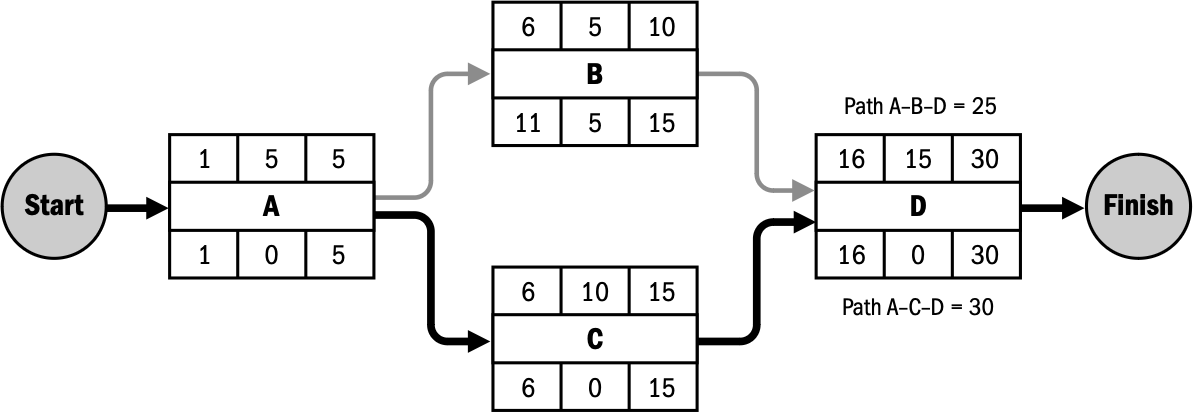
\includegraphics[width=\textwidth]{cpm-sample.png}
        \end{minipage}%
      };
    }
  {Gantt Chart}
  {Critical Path Method}
  {Project Schedule}
  {PERT Diagram}
  {diagram}

\pmbaQuestion
  {A customer asks you to complete the project one month faster. How can you do this, as a project manager?}
  {Smoothies and Free Snacks}
  {Carrots and Sticks}
  {Crashing and Fast Tracking}
  {Paying and Praying}
  {cpm, schedule-compression}

\pmbaQuestion
  {Which of the following belongs to the S.M.A.R.T. acronym (pick one)?}
  {Magnificent}
  {Ambitious}
  {Repetitive}
  {Time-boxed}
  {pdd}

\plush{
\pptBanner{Critical Path Method}\par
\pptPic{.8}{cpm.png}\par
{\scriptsize The picture is taken from \href{https://en.wikipedia.org/wiki/Critical_path_method}{Wikipedia}.\par}}

\plush{
  \pptBanner{Homework:}
  ``A \emph{Project Schedule} presents linked activities with planned dates, durations,
  milestones, and resources. At a minimum, the project schedule includes a planned start
  date and planned finish date for each activity. The project schedule presentation
  may be presented in summary form, sometimes referred to as the master schedule or
  milestone schedule, or presented in detail.''
  --- PMBOK5
}

\plush{
  \pptBanner{Read this:}
  Wikipedia:
    \href{https://en.wikipedia.org/wiki/Cone_of_Uncertainty}{Cone of Uncertainty},
    \href{https://en.wikipedia.org/wiki/Rolling-wave_planning}{Rolling-wave planning},
    \href{https://en.wikipedia.org/wiki/Three-point_estimation}{Three-point estimation},
    \href{https://en.wikipedia.org/wiki/COCOMO}{COCOMO}\par
  \href{http://www.technoparkcorp.com/process/cost/rom/}{Rough Order Of Magnitude Estimate} (2014)\par
  \href{https://www.yegor256.com/2020/11/03/daily-reports.html}{The Pain of Daily Reports} (2020)\par
  \href{https://www.yegor256.com/2015/01/08/morning-standup-meetings.html}{Daily Stand-Up Meetings Are a Good Tool for a Bad Manager} (2015)\par
  \href{https://www.yegor256.com/2019/09/03/injection-of-guilt.html}{Daily Stand-up Injection of Guilt}\par
  \href{https://www.yegor256.com/2015/06/02/how-to-estimate-software-cost.html}{How Much For This Software?} (2015)\par
}

\end{document}
